\chapter{Diversidad de rango}

Continuando con el estudio de las migraciones, los resultados del capitulo anterior han llevado a pesar en las migraciones como un conjunto con propiedades comunes, entre ellas que el uso de un idioma no se ve alterado por las palabras que conforman el corpus.   Otra propiedad se puede obtener al cuantificar qué tanto cambian las palabras que componen los préstamos de un idioma en otro, conforme avanza el tiempo. 
  
Como los préstamos entre idiomas están organizados por año, y a la vez en cada año se ordenan las palabras de forma ascendente por rango, (donde el rango más bajo corresponde a la palabra más utilizada en ese año y la de rango más alto a la menos utilizada), un mismo rango puede ser ocupado por diferentes palabras a lo largo del tiempo. 

Se define como \textbf{diversidad de rango} a la cantidad de elementos  diferentes que tienen un mismo rango en un mismo corpus. El algoritmo para llegar a la diversidad lo describe \textit{Sanchéz S.} \cite{tesis.sergio} de la siguiente manera:


\begin{enumerate}
		
	\item Se fijan un año inicial $t_{o}$ y uno final $t_{o}$, construyendo un intervalo de años a evaluar $\Delta\,t = t_{f}- t_{o}$.
	
	\item Se toma el primer rango de todos los años en el intervalo y se cuenta el número de palabras que son distintas en ese rango. Esta cantidad será la diversidad para el rango uno.
	
	\item Se prosigue con el segundo rango y se vuelve a contar cuántas palabras son diferentes en todo el periodo de tiempo.  Con ello se obtiene la diversidad para el rango dos. 
	
	\item Ya que las listas de préstamos de un idioma en otro no son homogéneas en cantidad, el procedimiento anterior se repetirá hasta el rango mínimo que poseen todas las listas,  así se asegura tener una homogeneidad en el tamaño.
	
	\item Se normalizan  los valores dividiendo cada resultado entre el número de años comprendidos del intervalo $\Delta\,t$, obteniendo  la diversidad de rango $d(k)$.
	
\end{enumerate}

La diversidad ha sido utilizada en corpus donde se clasifican las palabras más comunes de seis diferentes idiomas  por \textit{Cocho et al.} \cite{iplosone} y en  deportes y juegos  con diferentes criterios para establecer un orden por \textit{Morales et al.} \cite{epj}. En cada caso la diversidad es una característica común, por lo que se espera resultados similares al emplearla en el conjunto de los préstamos acumulados entre idiomas. 
 

%Tras graficar el rango contra la diversidad, se observó que en todas las combinaciones (a pesar de que algunas tuvieran más datos)  la tendencia de la diversidad  se asemeja a una función de distribución cumulativa logarítmica  normal, la cual depende del rango $k$, y la desviación estándar $\sigma$.

%\begin{equation}
%\label{ec.cumulativa}
%F(k) = \Phi \left ( \frac{ln(k)}{\sigma} \right )\,\,\,\,k\geq 0; \sigma \geq 0
%\end{equation}

%Donde $\Phi$ es la función cumulativa de la distribución normal, que ademas del rango y la desviación estándar, depende del promedio $\mu$.

%\begin{equation}
%\label{ec.distribucionnormal}
%\Phi(t) = \frac{1}{\sigma\sqrt{2\pi}} \int_{-\infty}^{t}  e^{ \frac{ - \left ( x-\mu \right )^{2}}{2\sigma^2}  } dx	
%\end{equation}



\section{Ajuste de datos}

Al graficar la diversidad de rango en las diferentes combinaciones de origen y receptor, la distribución de los valores asemejan a una curva logarítmica, sin embargo no son similares a las curvas sigmoides obtenidas  por \textit{Cocho et al} y  por \textit{Morales et al}, a pesar de seguir el mismo algoritmo.   

La principal diferencia con  los trabajos previos son los rangos donde se buscan la diversidad, estos llegan a ser del orden de $10^{4}$, mientras que en los préstamos acumulados  los rangos varían entre 8 y 290; siendo la escasez de rangos el factor que en este caso determina el obtener una curva logarítmica. 

Tomando en cuenta los puntos obtenidos para la diversidad $d(k)$, se propone que para los rangos $k$ la curva que mejor ajusta es de la forma

\begin{equation}
\label{ec.ajuste}
h(k) =  \alpha \, ln(k) + \beta
\end{equation}

Donde los parámetros $\alpha$ y $\beta$  se  obtienen por el método de mínimos cuadrados, entre los puntos obtenidos y la ecuación propuesta.  

%Donde los parámetros \alpha y \beta  se  obtienen por el método de mínimos cuadrados, minimizando la suma de los cuadrados de los errores, entre los puntos obtenidos y la ecuación propuesta. 


Para la fiabilidad del ajuste, se empleó el coeficiente de determinación $R^{2}$. Si $h_{k}$  representa el  valor de la ecuación de ajuste evaluada en el rango $k$,  $d_{k}$ es la diversidad obtenida para el mismo rango y $\bar{d}$ el promedio de todos los valores de la diversidad, entonces $R^{2}$ queda expresado como

\begin{equation}
\label{ec.r2_diversidad}
R^{2} = 1 - \sum_{k = 1} \frac{ \left( d_{k} - h_{k} \right)^{2}  }{ \left( d_{k} - \bar{d} \right)^{2} }	
\end{equation}

Al realizar la diversidad de rango de todas las combinaciones de idioma origen e idioma receptor,  se establecieron a $\alpha = 0.17\pm 0.04$ y $\beta = -0.18 \pm 0.08$, obtenidas a partir del promedio de cada $\alpha$ y $\beta$ tras el ajuste de cada combinación.  Si se sustituyen estos valores en la ecuación \ref{ec.ajuste}, la curva que mejor ajusta a la diversidad $d(k)$ es:


\begin{equation}
\label{ec.gen_ajs}
h(k) = 0.17\,ln(k) - 0.18
\end{equation} 

Se graficó la ecuación anterior junto a los valores de diversidad de rango de todas las combinaciones de idioma origen e idioma receptor, siendo mayor la diversidad conforme el rango $k$ se acerca a sus valores más altos.



\begin{figure}[h!]
	\centering
	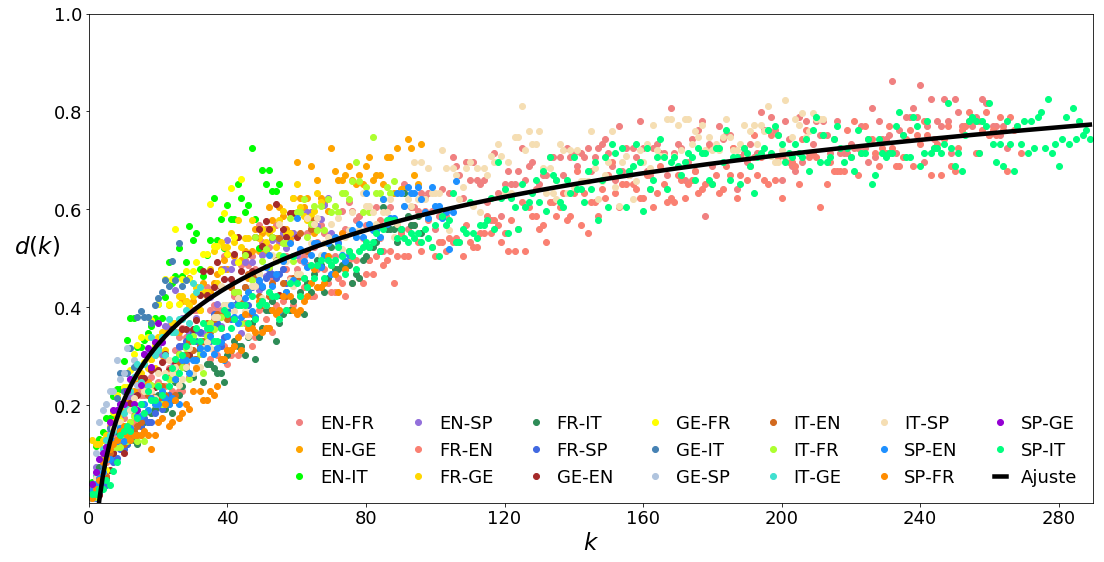
\includegraphics[scale=.38]{DR_gen.png}
	\label{fig.DR_gen}
	\caption{Diversidad de rango entre idiomas. La diversidad de rango $d(k)$ de las palabras migrantes ajustan a una curva logaritmica $h(k) = 0.17\,ln(k) - 0.18$, sin importar la cantidad de rangos que se utilicen. La mayor diversidad se encuentra conforme }
\end{figure}


A pesar de haber pocos rangos en algunas combinaciones, el ajuste fue optimo, ya que el coeficiente de determinación $R^{2}$ entre la diversidad y la nueva expresión del ajuste, tomó valores entre 0.79 y 0.95, correspondiendo las cifras mas bajas a las migraciones con escasez de rangos, principalmente en las combinaciones  del alemán con alguna lengua romance.  

%% dejo comentada la siguiente tabla por si se llega a necesitar algun dato

%\begin{table}[h!]
%	\centering
%	\begin{tabular}{ccccccc}
%		\textbf{}                & \textbf{$\mu$} & \textbf{$\sigma$} & \textbf{$k_{min}$} & \textbf{$\alpha$} & \textbf{$\beta$} & \textbf{$R^{2}$} \\
%		\textbf{inglés-francés}  & 0.61           & 0.18                & 265                   & 0.18           & -0.23         & 0.94        \\
%		\textbf{inglés-alemán}   & 0.49           & 0.19                & 96                    & 0.19           & -0.23         & 0.92        \\
%		\textbf{ingles-italiano} & 0.45           & 0.17                & 55                    & 0.17           & -0.10         & 0.91        \\
%		\textbf{ingles-español}  & 0.38           & 0.15                & 70                    & 0.15           & -0.14         & 0.88        \\
%		\textbf{francés-inglés}  & 0.55           & 0.18                & 269                   & 0.18           & -0.29         & 0.93        \\
%		\textbf{francés-alemán}   & 0.42           & 0.16                & 67                    & 0.17           & -0.12         & 0.87        \\
%		\textbf{francés-italiano} & 0.35           & 0.16                & 96                    & 0.15           & -0.21         & 0.83        \\
%		\textbf{francés-español}  & 0.28           & 0.14                & 57                    & 0.15           & -0.19         & 0.86        \\
%		\textbf{alemán-inglés}  & 0.35             & 0.17                & 60                    & 0.18           & -0.22         & 0.88        \\
%		\textbf{alemán-francés}   & 0.37           & 0.17                & 44                    & 0.19           & -0.16         & 0.89        \\
%		\textbf{alemán-italiano} & 0.31            & 0.15                & 28                    & 0.17           & -0.11         & 0.91        \\
%		\textbf{alemán-español}  & 0.22            & 0.08                & 14                    & 0.10           & -0.04         & 0.89        \\
%		\textbf{italiano-inglés} & 0.31          & 0.15                & 66                   & 0.15           & -0.18        & 0.86        \\
%		\textbf{italiano-francés} & 0.41           & 0.20                & 88                    & 0.20           & -0.28         & 0.85        \\
%		\textbf{italiano-alemán}  & 0.26           & 0.12                & 32                    & 0.13           & -0.08         & 0.91        \\
%		\textbf{italiano-español}  & 0.22          & 0.19                & 212                    & 0.20           & -0.28         & 0.92       \\
%		\textbf{español-inglés}  & 0.41          & 0.18                & 106                   & 0.18           & -0.25        & 0.87        \\
%		\textbf{español-francés}   & 0.28           & 0.14                & 75                   & 0.13           & -0.17         & 0.79        \\
%		\textbf{español-alemán} & 0.21           & 0.09                & 21                    & 0.11           & -0.02         & 0.86        \\
%		\textbf{español-italiano}  & 0.22          & 0.18                & 289                    & 0.18           & -0.28         & 0.95       
%	\end{tabular}
%	\caption{Parámetros de la diversidad entre idiomas.}
%	\label{tab.DR_EN}
%\end{table}


\section{La relación entre diversidad de rango y la ley de Zipf}

El proponer una curva logarítmica mostró una similitud con los puntos de la diversidad de rango, obteniendo valores de $R^{2}$ aceptables. 
 
La fiabilidad del ajuste llevó buscar un vínculo entre la ecuación propuesta y  la ley de Zipf [XXX]. Por un lado la ley de Zipf relaciona el rango de las palabras $k$ con su frecuencia de aparición $f(k)$,  mientras que la diversidad de rango $d(k) $cuantifica las distintas palabras que ocupan un mismo rango dentro de una escala temporal.  

El término clave en los dos procedimientos es el rango, esta cantidad es el medio por el cual establecer la relación a través de una integral.

Utilizando la ley de Zipf para rangos bajos (ya que los préstamos acumulados entre idiomas no contienen más de trescientos elementos)

\begin{equation}
\label{ec.Zipf_kbajos}
f(k)  =  \frac{1}{k} 
\end{equation} 


Si se multiplica la expresión por una constante $\alpha$ y se hace una integral indefinida sobre la variable k

\begin{equation}
\label{ec.Zipf_int}
\int \frac{\alpha}{k}\,\,dk \, = \, \alpha \, ln \left(k\right) + C
\end{equation} 

Si la constante de integración $C = \beta$, entonces se llega a la forma propuesta para la diversidad de rango $h(k)$.  

\begin{subequations}
	\begin{align}
	\label{ec.Zipf_dk}
	\int \alpha f\left(k\right) \,dk \,=\, h(k) \\
	\int \frac{\alpha}{k}\,\,dk \, = \, \alpha \, ln \left(k\right) + \beta	
	\end{align}
\end{subequations}


La relación entre ambas propuestas se pudo haber logrado partiendo de la ecuación de diversidad y con una derivada sobre el rango llegar a la ley de Zipf, sin embargo la razón de hacer la integral sobre la ley de Zipf es que esta ley  ha sido probada con diferentes datos, en cambio la ecuación logarítmica en la diversidad funcionó en conjuntos con $k$ bajos, cuya mayor diversidad se alcanza conforme $k$ se aproxima a sus valores más altos.  

En caso de tener distintos tipos de datos (que cumplan la ley de Zipf), con poca cantidad de rangos y cuya diversidad se ajuste a una ecuación logarítmica, daría veracidad a la relación anterior. Además podría mostrar a la diversidad de rango en un análogo con un potencial escalar, donde se concentre la información del sistema, y se obtengan otras magnitudes o propiedades a través  de operaciones o transformadas. 

 



